\normalfalse \difficiletrue \tdifficilefalse
\correctionfalse
%\UPSTIidClasse{11} % 11 sup, 12 spé
%\newcommand{\UPSTIidClasse}{12}

\exer{Borne réglable  $\star\star$ \label{CIN:01:B2:12:1018}}
\setcounter{question}{0}\marginnote{\xpComp{CIN}{01}}%\UPSTIcompetence{B2-12}
\index{Compétence B2-12}\index{Compétence CIN-01}
\index{Schéma cinématique}

\ifcorrection
\else
\marginnote{\textbf{Pas de corrigé pour cet exercice.}}
\fi

\ifprof
\else
Soit la borne réglable suivante. 
\begin{marginfigure}
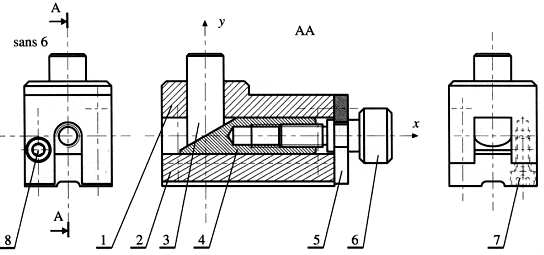
\includegraphics[width=\linewidth]{1018_01}
\end{marginfigure}
\fi


\ifprof
\else
La nomenclature est la suivante. 

\begin{marginfigure}
\begin{tabular}{lll}
\hline
\textbf{Rep} & \textbf{Désignation} & \textbf{Quantité} \\ \hline 
1 & Coulisseau & 1 \\ 
2 & Borne & 1 \\ 
3 & Corps & 1 \\ 
4 & Vis de guidage & 1 \\ 
5 & Couvercle & 1 \\ 
6 & Vis de couvercle & 2 \\ 
7 & Socle & 1 \\ 
8 & Vis de socle & 4 \\ 
10 & Molette & 1 \\ 
12 & Vis & 1 \\
13 & Goupille fendue & 1 \\ 
\hline
\end{tabular}
\end{marginfigure}
\fi


\question{Colorier le dessin de définition en utilisant la même couleur pour une même classe d'équivalence.}
\ifprof
\else
\fi

\question{Lister les classes classes d'équivalence.}
\ifprof
\else
\fi

\question{Donner le graphe de liaisons en précisant rigoureusement les liaisons. Justifier le choix des liaisons.}
\ifprof
\else
\fi


\question{Réaliser le schéma cinématique.}
\ifprof
\else
\fi

\ifprof
\else

\footnotesize
%\begin{marginfigure}
%\begin{tabular}{|p{.9\linewidth}|}
%\hline
%Indications (à vérifier...) :
%\begin{enumerate}
%\item $\vectv{B}{2}{0} = L\varphip(t)\vj{2} +\thetap(t)\left(L\vj{1}-R\vi{0}\right) $.
%\item  $\torseurcin{V}{2}{0} = \torseurl{\vecto{2}{0}=\left( \varphip(t)+\thetap(t) \right) \vk{0} }{ L\varphip(t)\vj{2} +\thetap(t)\left(L\vj{1}-R\vi{0}\right)}{B}$.
%\item $\vectg{B}{2}{0} =  L\varphipp(t)\vj{2}-L\varphip(t)\left(\varphip(t)+\thetap(t) \right)\vi{2}  + \thetapp(t)\left(L\vj{1}-R\vi{0}\right) - L\thetap^2(t)\vi{1}$.
%\end{enumerate} \\ \hline
%\end{tabular}
%\end{marginfigure}
\normalsize



\marginnote{Corrigé  voir \ref{CIN:01:B2:12:1018}.}

\fi